\documentclass[8pt,aspectratio=169]{beamer}
\usetheme{Madrid}
\usepackage{graphicx}
\usepackage{booktabs}
\usepackage{adjustbox}
\usepackage{multicol}
\usepackage{amsmath}
\usepackage{listings}
\usepackage{xcolor}

% Color definitions
\definecolor{mlblue}{RGB}{0,102,204}
\definecolor{mlpurple}{RGB}{51,51,178}
\definecolor{mllavender}{RGB}{173,173,224}
\definecolor{mllavender2}{RGB}{193,193,232}
\definecolor{mllavender3}{RGB}{204,204,235}
\definecolor{mllavender4}{RGB}{214,214,239}
\definecolor{mlorange}{RGB}{255, 127, 14}
\definecolor{mlgreen}{RGB}{44, 160, 44}
\definecolor{mlred}{RGB}{214, 39, 40}
\definecolor{mlgray}{RGB}{127, 127, 127}

% Additional colors for template compatibility
\definecolor{lightgray}{RGB}{240, 240, 240}
\definecolor{midgray}{RGB}{180, 180, 180}

% Code listing colors
\definecolor{codegreen}{rgb}{0,0.6,0}
\definecolor{codegray}{rgb}{0.5,0.5,0.5}
\definecolor{codepurple}{rgb}{0.58,0,0.82}
\definecolor{backcolour}{rgb}{0.95,0.95,0.95}

% Apply custom colors to Madrid theme
\setbeamercolor{palette primary}{bg=mllavender3,fg=mlpurple}
\setbeamercolor{palette secondary}{bg=mllavender2,fg=mlpurple}
\setbeamercolor{palette tertiary}{bg=mllavender,fg=white}
\setbeamercolor{palette quaternary}{bg=mlpurple,fg=white}

\setbeamercolor{structure}{fg=mlpurple}
\setbeamercolor{section in toc}{fg=mlpurple}
\setbeamercolor{subsection in toc}{fg=mlblue}
\setbeamercolor{title}{fg=mlpurple}
\setbeamercolor{frametitle}{fg=mlpurple,bg=mllavender3}
\setbeamercolor{block title}{bg=mllavender2,fg=mlpurple}
\setbeamercolor{block body}{bg=mllavender4,fg=black}

% Remove navigation symbols
\setbeamertemplate{navigation symbols}{}

% Clean itemize/enumerate
\setbeamertemplate{itemize items}[circle]
\setbeamertemplate{enumerate items}[default]

% Reduce margins for more content space
\setbeamersize{text margin left=5mm,text margin right=5mm}

% Code listing style
\lstdefinestyle{pythonstyle}{
    backgroundcolor=\color{backcolour},
    commentstyle=\color{codegreen},
    keywordstyle=\color{mlpurple},
    numberstyle=\tiny\color{codegray},
    stringstyle=\color{codepurple},
    basicstyle=\ttfamily\scriptsize,
    breakatwhitespace=false,
    breaklines=true,
    captionpos=b,
    keepspaces=true,
    numbers=left,
    numbersep=5pt,
    showspaces=false,
    showstringspaces=false,
    showtabs=false,
    tabsize=2,
    language=Python,
    frame=single,
    framerule=0.5pt,
    rulecolor=\color{mllavender}
}
\lstset{style=pythonstyle}

% Command for bottom annotation (Madrid-style)
\newcommand{\bottomnote}[1]{%
\vfill
\vspace{-2mm}
\textcolor{mllavender2}{\rule{\textwidth}{0.4pt}}
\vspace{1mm}
\footnotesize
\textbf{#1}
}

\title{Cryptography for Blockchain}
\subtitle{Lesson 2 of 4: Cryptocurrency \& Blockchain Development}
\author{Prof. Dr. Joerg Osterrieder}
\institute{University Lecture Series}
\date{\today}

\begin{document}

% ==================== SLIDE 1: TITLE ====================
\begin{frame}[plain]
\titlepage
\end{frame}

% ==================== SLIDE 2: OUTLINE ====================
\begin{frame}[t]{Lesson Outline}
\tableofcontents
\vfill
\footnotesize
\textbf{Duration:} 45 minutes | \textbf{Prerequisites:} Lesson 1 (Blockchain Fundamentals)
\end{frame}

% ==================== SECTION 1: HASH FUNCTIONS ====================
\section{Hash Functions}

% ==================== SLIDE 3: WHAT IS A HASH FUNCTION ====================
\begin{frame}[t]{What is a Hash Function?}
\begin{columns}[T]
\column{0.48\textwidth}
\textbf{Definition}

A hash function is a mathematical algorithm that:
\begin{itemize}
\item Takes input of \textbf{any size}
\item Produces output of \textbf{fixed size}
\item Acts as a ``digital fingerprint''
\end{itemize}

\vspace{0.5em}
\textbf{Analogy}

Like a fingerprint scanner:
\begin{itemize}
\item Every person $\rightarrow$ unique fingerprint
\item Every file $\rightarrow$ unique hash
\item Cannot reconstruct person from fingerprint
\end{itemize}

\column{0.48\textwidth}
\textbf{Mathematical Notation}

$$H: \{0,1\}^* \rightarrow \{0,1\}^n$$

\vspace{0.5em}
Where:
\begin{itemize}
\item $H$ = hash function
\item $\{0,1\}^*$ = arbitrary-length binary input
\item $\{0,1\}^n$ = fixed-length $n$-bit output
\end{itemize}

\vspace{0.5em}
\textbf{Example (SHA-256)}
\begin{itemize}
\item Input: ``Hello'' (5 bytes)
\item Output: 256 bits (32 bytes)
\item Always 64 hex characters
\end{itemize}
\end{columns}

\bottomnote{Hash functions are fundamental building blocks of blockchain security}
\end{frame}

% ==================== SLIDE 4: PROPERTIES OF HASH FUNCTIONS ====================
\begin{frame}[t]{Essential Properties of Cryptographic Hash Functions}
\begin{columns}[T]
\column{0.31\textwidth}
\textbf{1. Deterministic}

Same input $\rightarrow$ same output

\vspace{0.3em}
\begin{itemize}
\item Reproducible results
\item No randomness involved
\item Essential for verification
\end{itemize}

\vspace{0.3em}
$$H(x) = H(x) \text{ always}$$

\column{0.31\textwidth}
\textbf{2. One-Way (Pre-image Resistant)}

Cannot reverse the hash

\vspace{0.3em}
\begin{itemize}
\item Given $h = H(x)$
\item Infeasible to find $x$
\item Protects original data
\end{itemize}

\vspace{0.3em}
$$H(x) \rightarrow h \checkmark$$
$$h \rightarrow x \times$$

\column{0.31\textwidth}
\textbf{3. Collision-Resistant}

Hard to find two inputs with same hash

\vspace{0.3em}
\begin{itemize}
\item Given $x$, hard to find $y$
\item Where $H(x) = H(y)$
\item Ensures uniqueness
\end{itemize}

\vspace{0.3em}
$$P(H(x) = H(y)) \approx 0$$
\end{columns}

\vspace{1em}
\begin{center}
\begin{tabular}{lcc}
\toprule
\textbf{Property} & \textbf{Security Guarantee} & \textbf{Blockchain Use} \\
\midrule
Deterministic & Verification & Block validation \\
One-way & Data protection & Transaction privacy \\
Collision-resistant & Integrity & Unique block IDs \\
\bottomrule
\end{tabular}
\end{center}

\bottomnote{Breaking any of these properties would compromise blockchain security}
\end{frame}

% ==================== SLIDE 5: SHA-256 IN DETAIL ====================
\begin{frame}[t]{SHA-256: The Blockchain Standard}
\begin{columns}[T]
\column{0.48\textwidth}
\textbf{SHA-256 Specifications}

\begin{itemize}
\item \textbf{Name:} Secure Hash Algorithm 256-bit
\item \textbf{Family:} SHA-2 (designed by NSA)
\item \textbf{Output:} 256 bits = 32 bytes = 64 hex chars
\item \textbf{Block size:} 512 bits
\item \textbf{Rounds:} 64 compression rounds
\end{itemize}

\vspace{0.5em}
\textbf{Security Level}

\begin{itemize}
\item $2^{256}$ possible outputs
\item More than atoms in universe ($\approx 10^{80}$)
\item Brute force: infeasible
\item No known practical attacks
\end{itemize}

\column{0.48\textwidth}
\textbf{Example Hash}

\vspace{0.3em}
Input: \texttt{"Bitcoin"}

\vspace{0.3em}
SHA-256 Output:
\begin{center}
\footnotesize
\texttt{b4056df6691f8dc7...}\\
\texttt{...2e6d7c26c374ef0}
\end{center}

\vspace{0.5em}
\textbf{Why Bitcoin Uses SHA-256}

\begin{itemize}
\item Block header hashing
\item Merkle tree construction
\item Proof-of-Work puzzles
\item Address generation (with RIPEMD-160)
\end{itemize}
\end{columns}

\vspace{0.5em}
\begin{center}
\colorbox{mllavender4}{\parbox{0.8\textwidth}{\centering
\textbf{Fun Fact:} Bitcoin mining is essentially a race to find an input that produces a hash starting with many zeros.
}}
\end{center}
\end{frame}

% ==================== SLIDE 6: HASH FUNCTION FLOW CHART ====================
\begin{frame}[t]{Hash Function: How It Works}
\begin{center}
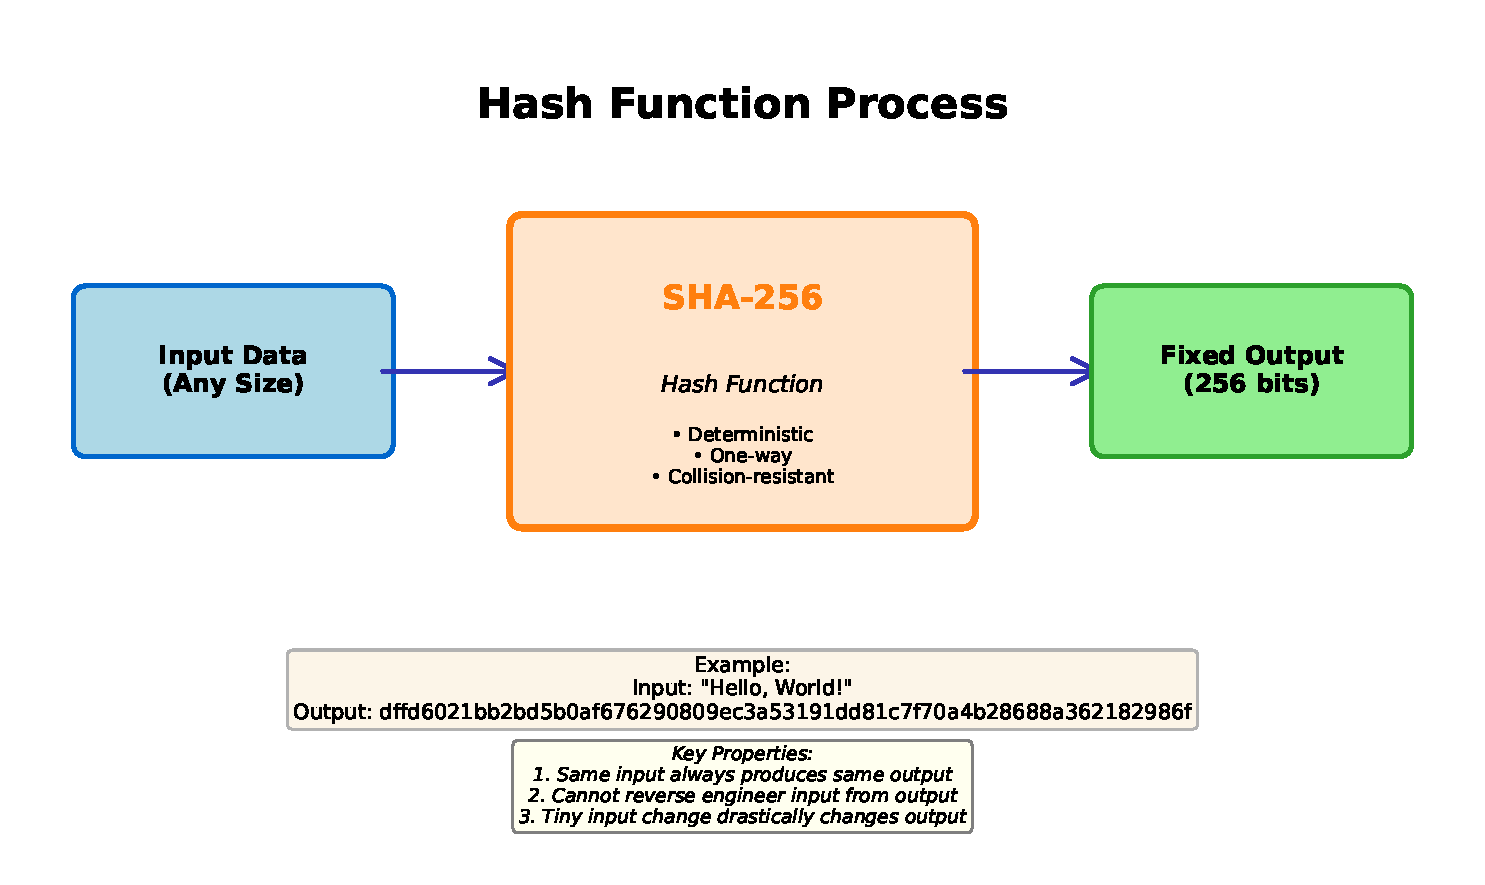
\includegraphics[width=0.85\textwidth]{01_hash_function/01_hash_function.pdf}
\end{center}

\bottomnote{The hash function processes input through multiple rounds to produce a fixed-size digest}
\end{frame}

% ==================== SLIDE 7: AVALANCHE EFFECT ====================
\begin{frame}[t]{The Avalanche Effect}
\begin{columns}[T]
\column{0.48\textwidth}
\textbf{Definition}

A small change in input causes a dramatic change in output.

\vspace{0.5em}
\textbf{Example}

Input 1: \texttt{"Hello, Blockchain!"}\\
Input 2: \texttt{"Hello, Blockchain."}\\
\footnotesize(Only difference: \texttt{!} vs \texttt{.})

\normalsize
\vspace{0.5em}
\textbf{Result}
\begin{itemize}
\item Completely different hashes
\item $\approx$50\% of bits change
\item No pattern or predictability
\end{itemize}

\column{0.48\textwidth}
\begin{center}
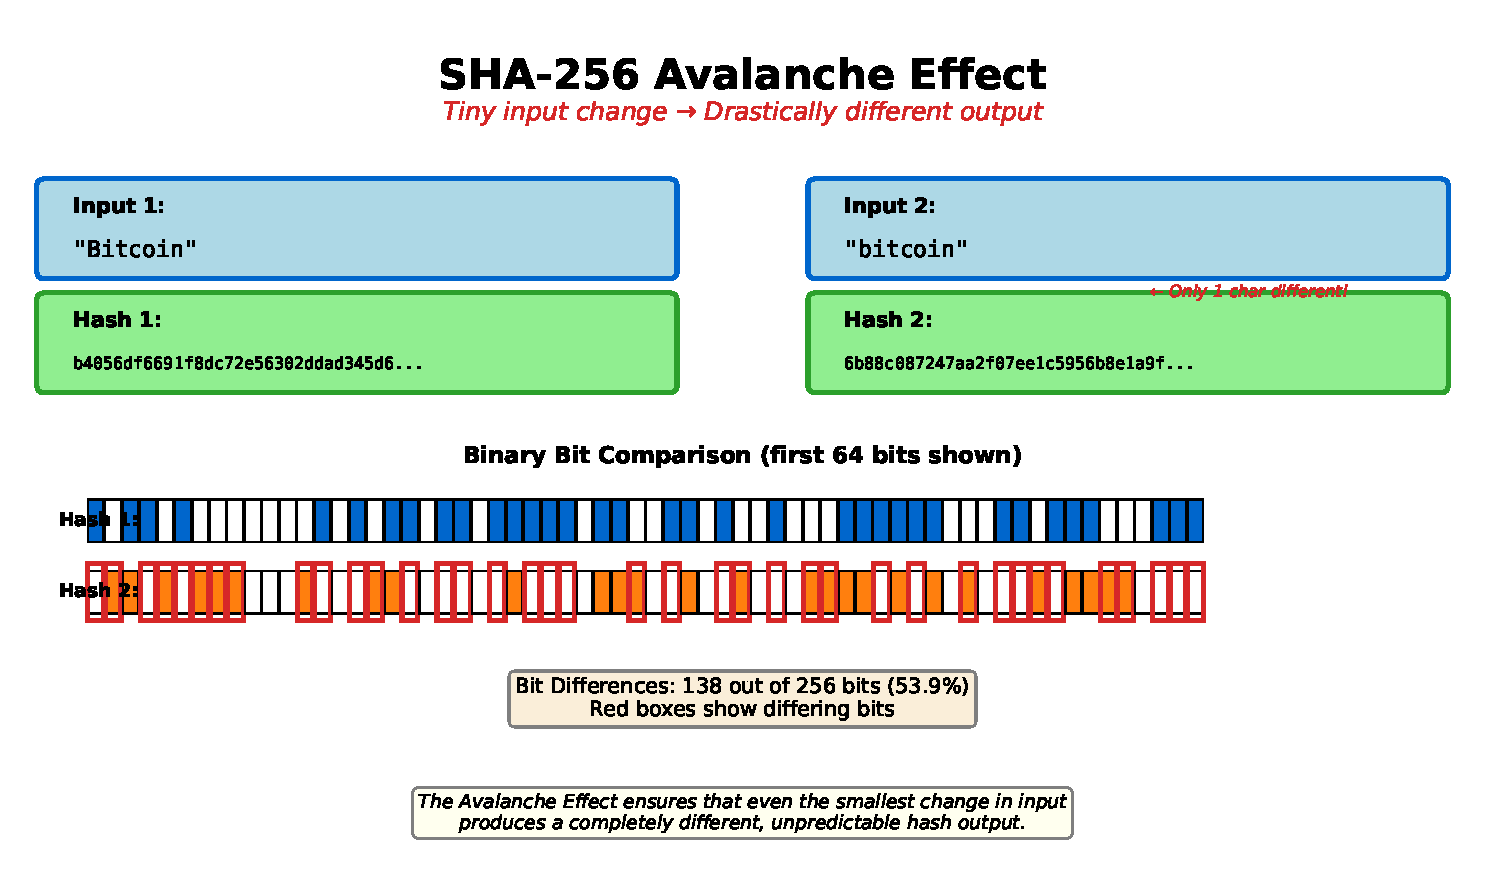
\includegraphics[width=\textwidth]{02_sha256_avalanche/02_sha256_avalanche.pdf}
\end{center}
\end{columns}

\vspace{0.5em}
\textbf{Why This Matters for Blockchain}
\begin{itemize}
\item[\textcolor{mlgreen}{+}] Tampering is immediately detectable
\item[\textcolor{mlgreen}{+}] Cannot predict hash without computing it
\item[\textcolor{mlgreen}{+}] Mining difficulty can be precisely controlled
\end{itemize}

\bottomnote{The avalanche effect ensures that even tiny modifications are immediately apparent}
\end{frame}

% ==================== SLIDE 8: CODE - PYTHON HASHING ====================
\begin{frame}[t,fragile]{Code Demo: Hashing in Python}
\begin{columns}[T]
\column{0.48\textwidth}
\textbf{Basic SHA-256 Hashing}

\begin{lstlisting}
import hashlib

def sha256_hash(data: str) -> str:
    """Compute SHA-256 hash."""
    return hashlib.sha256(
        data.encode()
    ).hexdigest()

# Example usage
text = "Hello, Blockchain!"
hash_value = sha256_hash(text)
print(f"Input: {text}")
print(f"Hash:  {hash_value}")
\end{lstlisting}

\column{0.48\textwidth}
\textbf{Demonstrating Avalanche Effect}

\begin{lstlisting}
text1 = "Hello, Blockchain!"
text2 = "Hello, Blockchain."

hash1 = sha256_hash(text1)
hash2 = sha256_hash(text2)

# Count differing bits
diff = bin(
    int(hash1, 16) ^ int(hash2, 16)
).count('1')

print(f"Bits changed: {diff}/256")
# Output: ~128 bits (50%)
\end{lstlisting}
\end{columns}

\vspace{0.5em}
\begin{center}
\colorbox{mllavender4}{\parbox{0.9\textwidth}{\centering
\textbf{Try it:} Run \texttt{python code/hashing\_demo.py} to see these examples in action
}}
\end{center}
\end{frame}

% ==================== SLIDE 9: WHY BLOCKCHAIN NEEDS HASHING ====================
\begin{frame}[t]{Why Blockchain Needs Hashing}
\begin{columns}[T]
\column{0.48\textwidth}
\textbf{Block Identification}

Each block has a unique hash:
\begin{itemize}
\item Block hash = fingerprint
\item Links to previous block
\item Creates immutable chain
\end{itemize}

\vspace{0.5em}
\textbf{Data Integrity}

\begin{itemize}
\item Hash of transactions (Merkle root)
\item Any change $\rightarrow$ different hash
\item Instant tamper detection
\end{itemize}

\column{0.48\textwidth}
\textbf{Proof-of-Work Mining}

\begin{itemize}
\item Find nonce where:
\item $H(\text{block}) < \text{target}$
\item Requires massive computation
\item Provides security
\end{itemize}

\vspace{0.5em}
\textbf{Address Generation}

\begin{itemize}
\item Public key $\rightarrow$ Hash $\rightarrow$ Address
\item Shorter, more manageable
\item Additional privacy layer
\end{itemize}
\end{columns}

\vspace{0.5em}
\begin{center}
\begin{tabular}{lcl}
\toprule
\textbf{Use Case} & \textbf{Hash Function} & \textbf{Purpose} \\
\midrule
Bitcoin blocks & SHA-256 (double) & Block ID \& PoW \\
Merkle trees & SHA-256 & Transaction verification \\
Bitcoin addresses & SHA-256 + RIPEMD-160 & Address derivation \\
Ethereum & Keccak-256 & All hashing operations \\
\bottomrule
\end{tabular}
\end{center}

\bottomnote{Without hash functions, blockchain integrity would be impossible to maintain}
\end{frame}

% ==================== SECTION 2: PUBLIC KEY CRYPTOGRAPHY ====================
\section{Public Key Cryptography}

% ==================== SLIDE 10: SYMMETRIC VS ASYMMETRIC ====================
\begin{frame}[t]{Symmetric vs. Asymmetric Encryption}
\begin{columns}[T]
\column{0.48\textwidth}
\textbf{Symmetric Encryption}

Same key for encrypt \& decrypt

\vspace{0.3em}
\begin{itemize}
\item[\textcolor{mlgreen}{+}] Fast and efficient
\item[\textcolor{mlgreen}{+}] Simple implementation
\item[\textcolor{mlorange}{-}] Key distribution problem
\item[\textcolor{mlorange}{-}] Need secure channel to share key
\end{itemize}

\vspace{0.3em}
\textbf{Examples:} AES, DES, ChaCha20

\vspace{0.3em}
$$E_k(m) = c \quad D_k(c) = m$$

\column{0.48\textwidth}
\textbf{Asymmetric Encryption}

Different keys: public \& private

\vspace{0.3em}
\begin{itemize}
\item[\textcolor{mlgreen}{+}] No key distribution problem
\item[\textcolor{mlgreen}{+}] Enables digital signatures
\item[\textcolor{mlorange}{-}] Slower than symmetric
\item[\textcolor{mlorange}{-}] Computationally intensive
\end{itemize}

\vspace{0.3em}
\textbf{Examples:} RSA, ECDSA, Ed25519

\vspace{0.3em}
$$E_{pub}(m) = c \quad D_{priv}(c) = m$$
\end{columns}

\vspace{1em}
\begin{center}
\colorbox{mllavender4}{\parbox{0.85\textwidth}{\centering
\textbf{Blockchain uses asymmetric cryptography} because users need to prove ownership without revealing their private keys to anyone.
}}
\end{center}

\bottomnote{Public key cryptography solved the key distribution problem that plagued symmetric encryption}
\end{frame}

% ==================== SLIDE 11: KEY PAIRS EXPLAINED ====================
\begin{frame}[t]{Understanding Key Pairs}
\begin{columns}[T]
\column{0.48\textwidth}
\textbf{Private Key}

\begin{itemize}
\item Secret number (256 bits for ECDSA)
\item Generated randomly
\item \textcolor{mlred}{\textbf{Never share!}}
\item Used to sign transactions
\item Proves ownership of funds
\end{itemize}

\vspace{0.3em}
\textbf{Think of it as:}
\begin{itemize}
\item Password to your bank vault
\item Master key to everything
\item Irreplaceable if lost
\end{itemize}

\column{0.48\textwidth}
\textbf{Public Key}

\begin{itemize}
\item Derived from private key
\item Can be shared freely
\item Used to verify signatures
\item Basis for wallet address
\item Cannot derive private key from it
\end{itemize}

\vspace{0.3em}
\textbf{Think of it as:}
\begin{itemize}
\item Your email address
\item Bank account number
\item Safe to share publicly
\end{itemize}
\end{columns}

\vspace{0.5em}
\begin{center}
\begin{tabular}{lcc}
\toprule
\textbf{Aspect} & \textbf{Private Key} & \textbf{Public Key} \\
\midrule
Visibility & Secret & Public \\
Purpose & Sign & Verify \\
Derivation & Random & From private key \\
Loss impact & Funds lost forever & None (regenerate) \\
\bottomrule
\end{tabular}
\end{center}
\end{frame}

% ==================== SLIDE 12: PUBLIC/PRIVATE KEY CHART ====================
\begin{frame}[t]{Public-Private Key Relationship}
\begin{center}
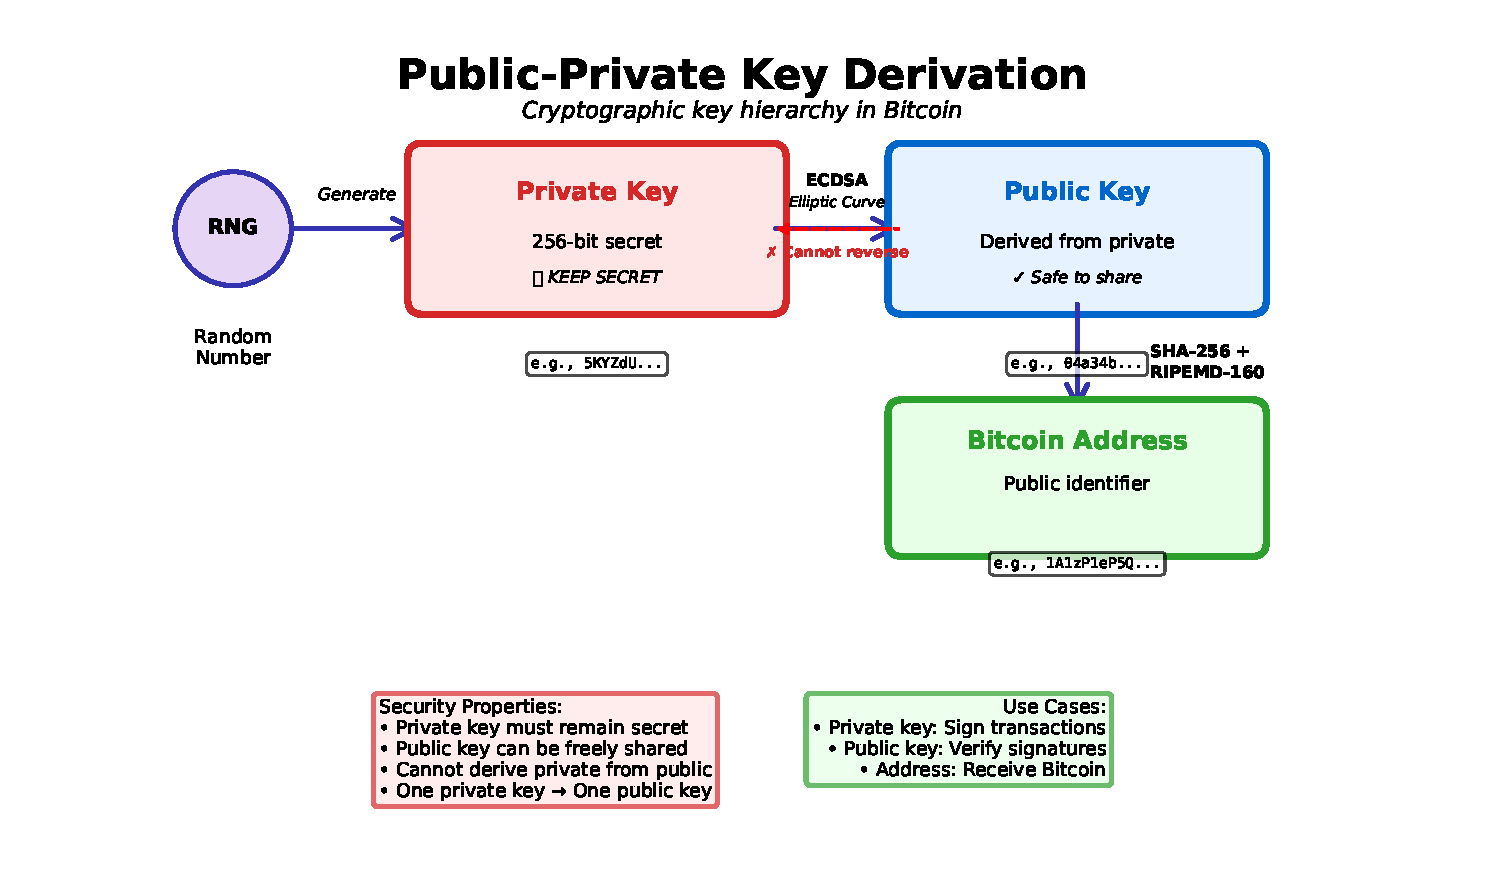
\includegraphics[width=0.9\textwidth]{03_public_private_keys/03_public_private_keys.pdf}
\end{center}

\bottomnote{The mathematical relationship between keys is based on elliptic curve mathematics}
\end{frame}

% ==================== SLIDE 13: HOW KEYS WORK IN BLOCKCHAIN ====================
\begin{frame}[t]{How Keys Work in Blockchain Transactions}
\begin{columns}[T]
\column{0.48\textwidth}
\textbf{Sending Cryptocurrency}

\begin{enumerate}
\item Create transaction message
\item Sign with \textbf{private key}
\item Broadcast to network
\item Miners verify with \textbf{public key}
\item Transaction added to block
\end{enumerate}

\vspace{0.5em}
\textbf{Why This Works}
\begin{itemize}
\item Only private key holder can sign
\item Anyone can verify with public key
\item Proves ownership without revealing key
\end{itemize}

\column{0.48\textwidth}
\textbf{Receiving Cryptocurrency}

\begin{enumerate}
\item Share your \textbf{address} (derived from public key)
\item Sender creates transaction to your address
\item Transaction references your public key
\item Only you can spend (with private key)
\end{enumerate}

\vspace{0.5em}
\textbf{Security Model}
\begin{itemize}
\item No central authority needed
\item Math guarantees authenticity
\item Cryptographic proof of ownership
\end{itemize}
\end{columns}

\vspace{0.5em}
\begin{center}
\colorbox{mllavender4}{\parbox{0.85\textwidth}{\centering
\textbf{Key Insight:} The blockchain never stores private keys. It only records transactions signed by private keys and verifiable by public keys.
}}
\end{center}
\end{frame}

% ==================== SLIDE 14: ELLIPTIC CURVE CRYPTOGRAPHY ====================
\begin{frame}[t]{Elliptic Curve Cryptography (ECC)}
\begin{columns}[T]
\column{0.48\textwidth}
\textbf{What is ECC?}

Mathematical system based on elliptic curves:
$$y^2 = x^3 + ax + b$$

\vspace{0.3em}
\textbf{Why Blockchain Uses ECC}
\begin{itemize}
\item Smaller keys than RSA
\item Same security level
\item Faster operations
\item Less storage needed
\end{itemize}

\vspace{0.3em}
\textbf{Security Comparison}
\begin{center}
\footnotesize
\begin{tabular}{cc}
\toprule
RSA & ECC \\
\midrule
3072 bits & 256 bits \\
7680 bits & 384 bits \\
\bottomrule
\end{tabular}
\end{center}

\column{0.48\textwidth}
\textbf{SECP256k1 Curve}

Used by Bitcoin \& Ethereum:
\begin{itemize}
\item $a = 0$, $b = 7$
\item $y^2 = x^3 + 7$
\item 256-bit keys
\item Not NSA-designed (transparency)
\end{itemize}

\vspace{0.3em}
\textbf{Key Generation (Simplified)}
\begin{enumerate}
\item Choose random private key $d$
\item Compute public key $Q = d \times G$
\item $G$ = generator point on curve
\item Reverse computation infeasible
\end{enumerate}
\end{columns}

\vspace{0.5em}
\bottomnote{ECC provides equivalent security to RSA with much smaller key sizes, making it ideal for blockchain}
\end{frame}

% ==================== SLIDE 15: CODE - KEY GENERATION ====================
\begin{frame}[t,fragile]{Code Demo: Key Generation in Python}
\begin{columns}[T]
\column{0.48\textwidth}
\textbf{Generate ECDSA Key Pair}

\begin{lstlisting}
from ecdsa import SigningKey, SECP256k1

def create_keypair():
    """Generate new key pair."""
    # Private key (random)
    private_key = SigningKey.generate(
        curve=SECP256k1
    )

    # Public key (derived)
    public_key = private_key.get_verifying_key()

    return private_key, public_key

# Generate keys
priv, pub = create_keypair()
print(f"Private: {priv.to_string().hex()}")
print(f"Public:  {pub.to_string().hex()}")
\end{lstlisting}

\column{0.48\textwidth}
\textbf{Key Properties}

\begin{lstlisting}
# Private key: 32 bytes (256 bits)
private_hex = priv.to_string().hex()
print(f"Length: {len(private_hex)} hex chars")
# Output: 64 hex chars

# Public key: 64 bytes (512 bits)
# (uncompressed: x + y coordinates)
public_hex = pub.to_string().hex()
print(f"Length: {len(public_hex)} hex chars")
# Output: 128 hex chars

# Compressed public key: 33 bytes
# (x coordinate + parity flag)
\end{lstlisting}

\vspace{0.5em}
\textbf{Required Library}
\begin{lstlisting}
pip install ecdsa
\end{lstlisting}
\end{columns}
\end{frame}

% ==================== SLIDE 16: SECURITY CONSIDERATIONS ====================
\begin{frame}[t]{Security Considerations}
\begin{columns}[T]
\column{0.48\textwidth}
\textbf{Random Number Generation}

\begin{itemize}
\item[\textcolor{mlred}{!}] Private key must be truly random
\item[\textcolor{mlred}{!}] Poor RNG = compromised security
\item[\textcolor{mlgreen}{\checkmark}] Use cryptographic RNG
\item[\textcolor{mlgreen}{\checkmark}] Hardware entropy sources
\end{itemize}

\vspace{0.5em}
\textbf{Key Storage Risks}
\begin{itemize}
\item Digital theft (malware, hacking)
\item Physical theft (device stolen)
\item Loss (hardware failure, forgotten)
\item Social engineering attacks
\end{itemize}

\column{0.48\textwidth}
\textbf{Best Practices}

\begin{itemize}
\item[\textcolor{mlgreen}{\checkmark}] Use hardware wallets for large amounts
\item[\textcolor{mlgreen}{\checkmark}] Backup seed phrases securely
\item[\textcolor{mlgreen}{\checkmark}] Use strong encryption
\item[\textcolor{mlgreen}{\checkmark}] Enable 2FA where possible
\item[\textcolor{mlgreen}{\checkmark}] Verify addresses before sending
\end{itemize}

\vspace{0.5em}
\textbf{Quantum Computing Threat}
\begin{itemize}
\item Shor's algorithm threatens ECC
\item Post-quantum cryptography emerging
\item Bitcoin/Ethereum monitoring this
\end{itemize}
\end{columns}

\vspace{0.5em}
\begin{center}
\colorbox{mllavender4}{\parbox{0.85\textwidth}{\centering
\textbf{Remember:} ``Not your keys, not your coins.'' Self-custody requires understanding and responsibility.
}}
\end{center}
\end{frame}

% ==================== SECTION 3: DIGITAL SIGNATURES ====================
\section{Digital Signatures}

% ==================== SLIDE 17: WHAT IS A DIGITAL SIGNATURE ====================
\begin{frame}[t]{What is a Digital Signature?}
\begin{columns}[T]
\column{0.48\textwidth}
\textbf{Definition}

A mathematical scheme that:
\begin{itemize}
\item Proves message authenticity
\item Verifies sender identity
\item Ensures message integrity
\item Provides non-repudiation
\end{itemize}

\vspace{0.5em}
\textbf{Real-World Analogy}

Like a handwritten signature but:
\begin{itemize}
\item Cannot be forged (mathematically)
\item Tied to specific message
\item Can be verified by anyone
\item Different for each message
\end{itemize}

\column{0.48\textwidth}
\textbf{Components}

\begin{enumerate}
\item \textbf{Key Generation:} Create key pair
\item \textbf{Signing:} $\sigma = Sign(sk, m)$
\item \textbf{Verification:} $Verify(pk, m, \sigma)$
\end{enumerate}

\vspace{0.5em}
\textbf{Properties}
\begin{itemize}
\item Only private key holder can sign
\item Anyone with public key can verify
\item Signature is unique to message
\item Cannot extract private key from signature
\end{itemize}
\end{columns}

\vspace{0.5em}
\begin{center}
\begin{tabular}{lcc}
\toprule
\textbf{Property} & \textbf{Physical Signature} & \textbf{Digital Signature} \\
\midrule
Forgery resistance & Low & Very high \\
Message binding & No & Yes \\
Verification & Subjective & Mathematical \\
\bottomrule
\end{tabular}
\end{center}
\end{frame}

% ==================== SLIDE 18: WHY TRANSACTIONS NEED SIGNATURES ====================
\begin{frame}[t]{Why Blockchain Transactions Need Signatures}
\begin{columns}[T]
\column{0.48\textwidth}
\textbf{Authorization Without Trust}

In traditional finance:
\begin{itemize}
\item Bank verifies your identity
\item PIN/password authenticates
\item Centralized trust model
\end{itemize}

\vspace{0.3em}
In blockchain:
\begin{itemize}
\item No central authority
\item Signature proves ownership
\item Math replaces trust
\end{itemize}

\vspace{0.3em}
\textbf{What Gets Signed}
\begin{itemize}
\item Sender address
\item Recipient address
\item Amount to transfer
\item Transaction metadata
\end{itemize}

\column{0.48\textwidth}
\textbf{Protection Provided}

\begin{itemize}
\item[\textcolor{mlgreen}{\checkmark}] \textbf{Authentication:} Proves sender identity
\item[\textcolor{mlgreen}{\checkmark}] \textbf{Integrity:} Detects tampering
\item[\textcolor{mlgreen}{\checkmark}] \textbf{Non-repudiation:} Cannot deny sending
\item[\textcolor{mlgreen}{\checkmark}] \textbf{Authorization:} Only owner can spend
\end{itemize}

\vspace{0.5em}
\textbf{Without Signatures}
\begin{itemize}
\item[\textcolor{mlred}{$\times$}] Anyone could spend your coins
\item[\textcolor{mlred}{$\times$}] No proof of transaction origin
\item[\textcolor{mlred}{$\times$}] Easy to forge transactions
\item[\textcolor{mlred}{$\times$}] Blockchain would be useless
\end{itemize}
\end{columns}

\bottomnote{Digital signatures are the foundation of ownership in decentralized systems}
\end{frame}

% ==================== SLIDE 19: ECDSA ALGORITHM ====================
\begin{frame}[t]{ECDSA: Elliptic Curve Digital Signature Algorithm}
\begin{columns}[T]
\column{0.48\textwidth}
\textbf{Signing Process}

Given message $m$ and private key $d$:
\begin{enumerate}
\item Compute $e = Hash(m)$
\item Select random $k$
\item Calculate point $(x_1, y_1) = k \times G$
\item Compute $r = x_1 \mod n$
\item Compute $s = k^{-1}(e + d \cdot r) \mod n$
\item Signature = $(r, s)$
\end{enumerate}

\vspace{0.3em}
\textbf{Output}
\begin{itemize}
\item Two 256-bit numbers: $r$ and $s$
\item Total signature: 64 bytes
\item Unique for each message
\end{itemize}

\column{0.48\textwidth}
\textbf{Verification Process}

Given message $m$, signature $(r, s)$, public key $Q$:
\begin{enumerate}
\item Compute $e = Hash(m)$
\item Compute $u_1 = e \cdot s^{-1} \mod n$
\item Compute $u_2 = r \cdot s^{-1} \mod n$
\item Calculate $(x_1, y_1) = u_1 \times G + u_2 \times Q$
\item Valid if $r = x_1 \mod n$
\end{enumerate}

\vspace{0.3em}
\textbf{Security Basis}
\begin{itemize}
\item Discrete logarithm problem
\item Cannot find $d$ from $Q = d \times G$
\end{itemize}
\end{columns}

\vspace{0.3em}
\begin{center}
\colorbox{mllavender4}{\parbox{0.85\textwidth}{\centering
\textbf{Note:} The random value $k$ must be truly random and unique for each signature. Reusing $k$ can leak the private key!
}}
\end{center}
\end{frame}

% ==================== SLIDE 20: SIGN/VERIFY FLOW CHART ====================
\begin{frame}[t]{Digital Signature Flow}
\begin{center}
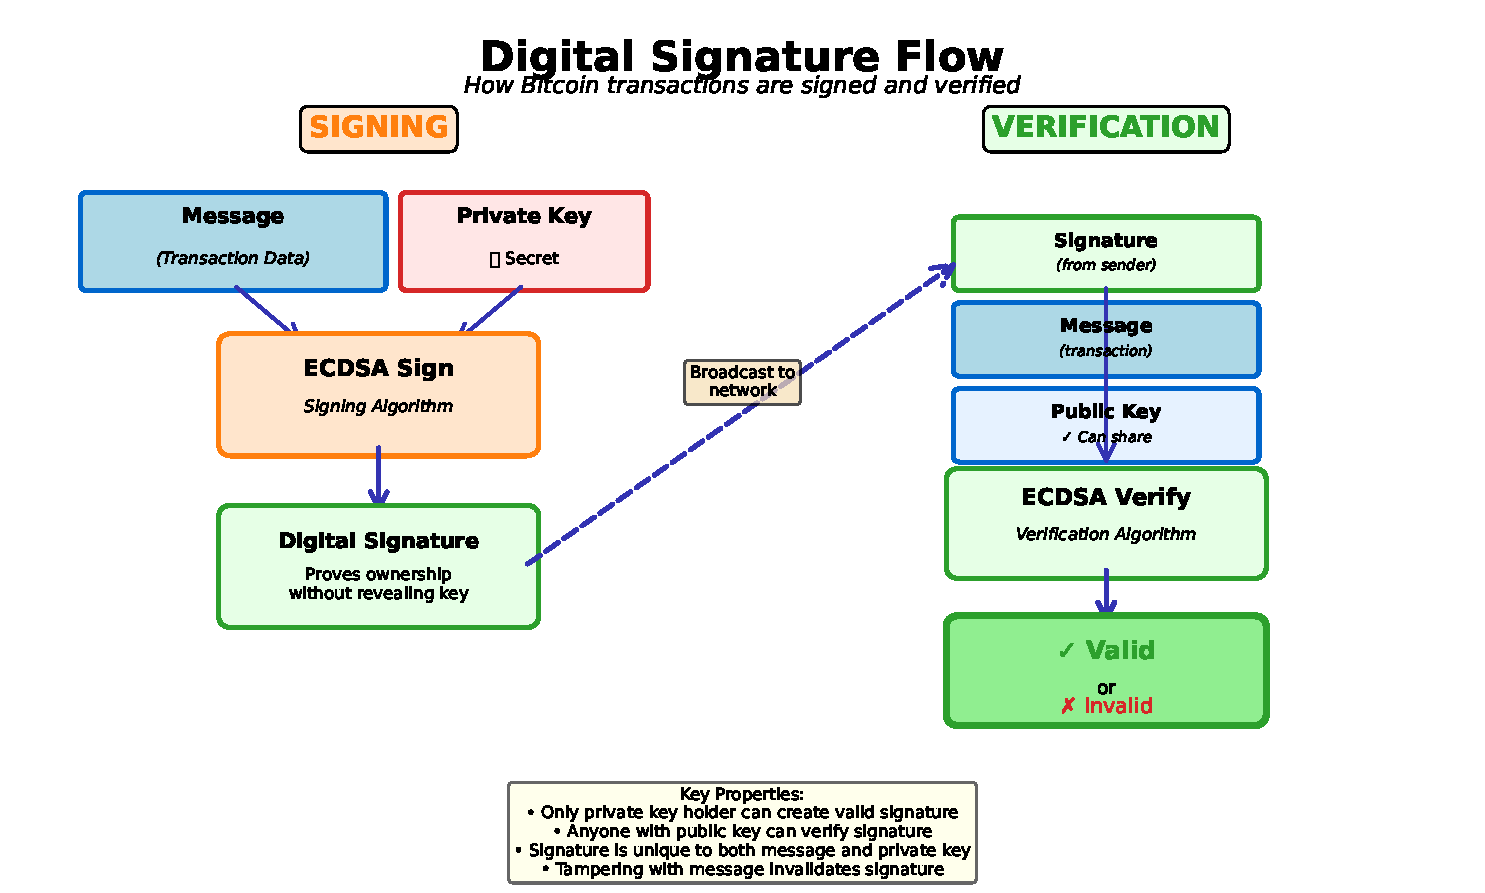
\includegraphics[width=0.9\textwidth]{04_digital_signature_flow/04_digital_signature_flow.pdf}
\end{center}

\bottomnote{The signing process uses the private key; verification uses only the public key}
\end{frame}

% ==================== SLIDE 21: CODE - SIGNING A MESSAGE ====================
\begin{frame}[t,fragile]{Code Demo: Signing a Message}
\begin{columns}[T]
\column{0.48\textwidth}
\textbf{Create Signature}

\begin{lstlisting}
from ecdsa import SigningKey, SECP256k1
import hashlib

def sign_message(private_key, message):
    """Sign a message with ECDSA."""
    # Hash the message
    msg_hash = hashlib.sha256(
        message.encode()
    ).digest()

    # Sign the hash
    signature = private_key.sign_digest(
        msg_hash
    )

    return signature
\end{lstlisting}

\column{0.48\textwidth}
\textbf{Usage Example}

\begin{lstlisting}
# Generate key pair
private_key = SigningKey.generate(
    curve=SECP256k1
)

# Message to sign
message = "Transfer 10 BTC to Alice"

# Create signature
signature = sign_message(
    private_key,
    message
)

print(f"Message: {message}")
print(f"Signature: {signature.hex()}")
# Signature: 64 bytes (r + s)
\end{lstlisting}
\end{columns}

\vspace{0.5em}
\begin{center}
\colorbox{mllavender4}{\parbox{0.9\textwidth}{\centering
\textbf{Important:} The signature is unique to this specific message. Changing even one character would require a new signature.
}}
\end{center}
\end{frame}

% ==================== SLIDE 22: CODE - VERIFYING A SIGNATURE ====================
\begin{frame}[t,fragile]{Code Demo: Verifying a Signature}
\begin{columns}[T]
\column{0.48\textwidth}
\textbf{Verification Function}

\begin{lstlisting}
from ecdsa import BadSignatureError

def verify_signature(public_key,
                     message,
                     signature):
    """Verify ECDSA signature."""
    try:
        msg_hash = hashlib.sha256(
            message.encode()
        ).digest()

        public_key.verify_digest(
            signature,
            msg_hash
        )
        return True
    except BadSignatureError:
        return False
\end{lstlisting}

\column{0.48\textwidth}
\textbf{Testing Verification}

\begin{lstlisting}
# Get public key from private key
public_key = private_key.get_verifying_key()

# Verify original message
is_valid = verify_signature(
    public_key, message, signature
)
print(f"Original: {is_valid}")  # True

# Try tampered message
tampered = "Transfer 100 BTC to Alice"
is_valid = verify_signature(
    public_key, tampered, signature
)
print(f"Tampered: {is_valid}")  # False

# Try wrong public key
wrong_pk = SigningKey.generate(
    curve=SECP256k1
).get_verifying_key()
is_valid = verify_signature(
    wrong_pk, message, signature
)
print(f"Wrong key: {is_valid}")  # False
\end{lstlisting}
\end{columns}
\end{frame}

% ==================== SLIDE 23: NON-REPUDIATION ====================
\begin{frame}[t]{Non-Repudiation: The Legal Power of Signatures}
\begin{columns}[T]
\column{0.48\textwidth}
\textbf{What is Non-Repudiation?}

The inability to deny having performed an action.

\vspace{0.5em}
\textbf{In Blockchain Context}
\begin{itemize}
\item Cannot deny signing a transaction
\item Signature proves you authorized it
\item Recorded permanently on chain
\item Cryptographic evidence
\end{itemize}

\vspace{0.5em}
\textbf{Why It Matters}
\begin{itemize}
\item Legal accountability
\item Dispute resolution
\item Audit trails
\item Trust without intermediaries
\end{itemize}

\column{0.48\textwidth}
\textbf{How It Works}

\begin{enumerate}
\item Only you have your private key
\item Only private key can create valid signature
\item Signature is publicly verifiable
\item Therefore: you must have signed it
\end{enumerate}

\vspace{0.5em}
\textbf{Implications}
\begin{itemize}
\item[\textcolor{mlred}{!}] Key theft = transaction theft
\item[\textcolor{mlred}{!}] No ``undo'' or ``cancel''
\item[\textcolor{mlred}{!}] No ``I forgot my password'' recovery
\item[\textcolor{mlgreen}{\checkmark}] Full control of your assets
\item[\textcolor{mlgreen}{\checkmark}] No middleman needed
\end{itemize}
\end{columns}

\vspace{0.5em}
\begin{center}
\colorbox{mllavender4}{\parbox{0.85\textwidth}{\centering
\textbf{Legal Note:} In many jurisdictions, digital signatures have the same legal standing as handwritten signatures for contracts and agreements.
}}
\end{center}
\end{frame}

% ==================== SECTION 4: WALLETS ====================
\section{Cryptocurrency Wallets}

% ==================== SLIDE 24: WALLET ARCHITECTURE ====================
\begin{frame}[t]{Wallet Architecture}
\begin{center}
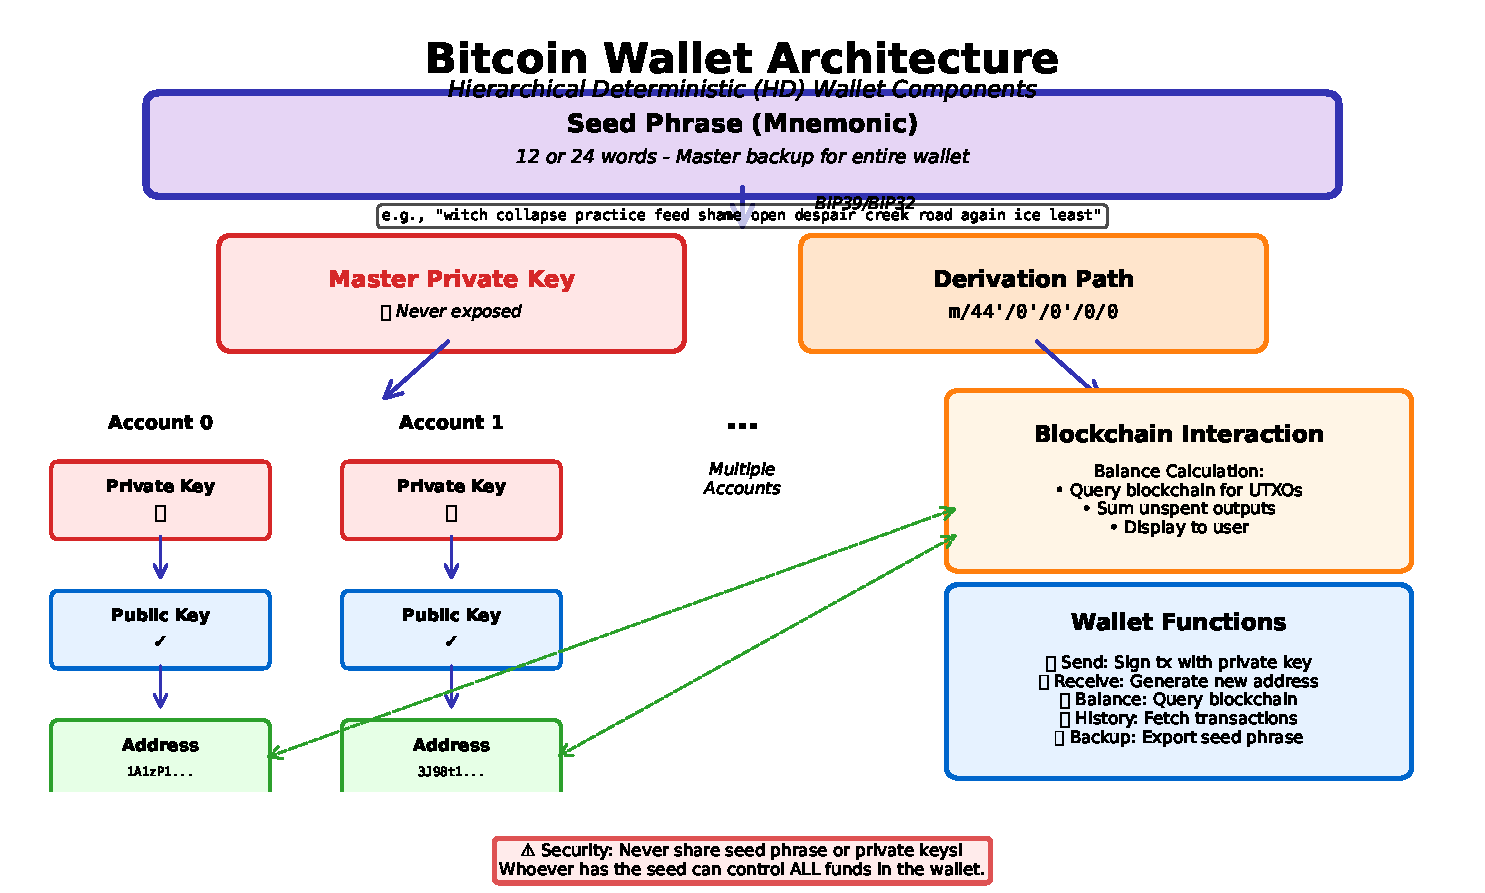
\includegraphics[width=0.85\textwidth]{05_wallet_architecture/05_wallet_architecture.pdf}
\end{center}

\bottomnote{A wallet is essentially a key management system, not a container for coins}
\end{frame}

% ==================== SLIDE 25: FROM SEED TO ADDRESS ====================
\begin{frame}[t]{From Seed Phrase to Wallet Address}
\begin{columns}[T]
\column{0.48\textwidth}
\textbf{The Derivation Chain}

\begin{enumerate}
\item \textbf{Entropy} (128-256 bits)\\
      Random data from secure source
\item \textbf{Mnemonic Seed} (12-24 words)\\
      Human-readable backup (BIP-39)
\item \textbf{Seed} (512 bits)\\
      PBKDF2 stretch of mnemonic
\item \textbf{Master Key}\\
      Root of HD wallet tree (BIP-32)
\item \textbf{Child Keys}\\
      Derived for each address
\item \textbf{Public Key}\\
      From private key (ECC)
\item \textbf{Address}\\
      Hash of public key
\end{enumerate}

\column{0.48\textwidth}
\textbf{Example Seed Phrase}

\footnotesize
\texttt{abandon abandon abandon abandon abandon abandon abandon abandon abandon abandon abandon about}
\normalsize

\vspace{0.5em}
\textbf{Why Seed Phrases?}
\begin{itemize}
\item[\textcolor{mlgreen}{\checkmark}] Human-readable backup
\item[\textcolor{mlgreen}{\checkmark}] Generate unlimited addresses
\item[\textcolor{mlgreen}{\checkmark}] Restore entire wallet
\item[\textcolor{mlgreen}{\checkmark}] Standardized (works across wallets)
\end{itemize}

\vspace{0.5em}
\textbf{Security Warning}
\begin{itemize}
\item[\textcolor{mlred}{!}] Anyone with seed phrase owns your funds
\item[\textcolor{mlred}{!}] Store offline, never digitally
\item[\textcolor{mlred}{!}] Use metal backup for fire/water protection
\end{itemize}
\end{columns}
\end{frame}

% ==================== SLIDE 26: CODE - GENERATE WALLET ====================
\begin{frame}[t,fragile]{Code Demo: Generate Wallet Address}
\begin{columns}[T]
\column{0.48\textwidth}
\textbf{Key Generation}

\begin{lstlisting}
from ecdsa import SigningKey, SECP256k1
import hashlib

def generate_keypair():
    """Generate ECDSA key pair."""
    private = SigningKey.generate(
        curve=SECP256k1
    )
    public = private.get_verifying_key()
    return (
        private.to_string().hex(),
        public.to_string().hex()
    )

priv_key, pub_key = generate_keypair()
print(f"Private Key: {priv_key}")
print(f"Public Key:  {pub_key}")
\end{lstlisting}

\column{0.48\textwidth}
\textbf{Address Derivation (Ethereum-style)}

\begin{lstlisting}
def derive_address(public_key_hex):
    """Derive address from public key."""
    # Convert to bytes
    pub_bytes = bytes.fromhex(
        public_key_hex
    )

    # Hash with Keccak-256 (simplified)
    # Using SHA-256 for demo
    hash_digest = hashlib.sha256(
        pub_bytes
    ).digest()

    # Take last 20 bytes, add 0x
    address = '0x' + hash_digest[-20:].hex()
    return address

address = derive_address(pub_key)
print(f"Address: {address}")
# Example: 0x7a250d5630b4cf539739df...
\end{lstlisting}
\end{columns}

\vspace{0.3em}
\begin{center}
\colorbox{mllavender4}{\parbox{0.9\textwidth}{\centering
\textbf{Try it:} Run \texttt{python code/wallet\_demo.py} for the complete demonstration
}}
\end{center}
\end{frame}

% ==================== SLIDE 27: HOT VS COLD WALLETS ====================
\begin{frame}[t]{Hot Wallets vs. Cold Wallets}
\begin{columns}[T]
\column{0.48\textwidth}
\textbf{Hot Wallets}

Connected to the internet

\vspace{0.3em}
\textbf{Types:}
\begin{itemize}
\item Mobile apps (Trust Wallet, Metamask Mobile)
\item Browser extensions (Metamask, Phantom)
\item Exchange wallets (Coinbase, Binance)
\item Desktop wallets (Exodus, Electrum)
\end{itemize}

\vspace{0.3em}
\textbf{Characteristics:}
\begin{itemize}
\item[\textcolor{mlgreen}{+}] Convenient for daily use
\item[\textcolor{mlgreen}{+}] Easy transactions
\item[\textcolor{mlorange}{-}] Vulnerable to hacks
\item[\textcolor{mlorange}{-}] Malware risk
\end{itemize}

\column{0.48\textwidth}
\textbf{Cold Wallets}

Offline storage

\vspace{0.3em}
\textbf{Types:}
\begin{itemize}
\item Hardware wallets (Ledger, Trezor)
\item Paper wallets (printed keys)
\item Air-gapped computers
\item Steel/metal backups
\end{itemize}

\vspace{0.3em}
\textbf{Characteristics:}
\begin{itemize}
\item[\textcolor{mlgreen}{+}] Maximum security
\item[\textcolor{mlgreen}{+}] Immune to online attacks
\item[\textcolor{mlorange}{-}] Less convenient
\item[\textcolor{mlorange}{-}] Physical security needed
\end{itemize}
\end{columns}

\vspace{0.5em}
\begin{center}
\begin{tabular}{lcc}
\toprule
\textbf{Use Case} & \textbf{Recommended} & \textbf{Amount} \\
\midrule
Daily spending & Hot wallet & Small amounts \\
Short-term trading & Hot wallet & Medium amounts \\
Long-term holding & Cold wallet & Large amounts \\
Inheritance planning & Cold + documentation & Any amount \\
\bottomrule
\end{tabular}
\end{center}
\end{frame}

% ==================== SLIDE 28: SECURITY BEST PRACTICES ====================
\begin{frame}[t]{Wallet Security Best Practices}
\begin{columns}[T]
\column{0.48\textwidth}
\textbf{Seed Phrase Protection}

\begin{itemize}
\item[\textcolor{mlgreen}{\checkmark}] Write on paper immediately
\item[\textcolor{mlgreen}{\checkmark}] Store in multiple locations
\item[\textcolor{mlgreen}{\checkmark}] Consider metal backup
\item[\textcolor{mlred}{$\times$}] Never store digitally
\item[\textcolor{mlred}{$\times$}] Never screenshot
\item[\textcolor{mlred}{$\times$}] Never email/message
\end{itemize}

\vspace{0.5em}
\textbf{Transaction Safety}

\begin{itemize}
\item[\textcolor{mlgreen}{\checkmark}] Always verify addresses
\item[\textcolor{mlgreen}{\checkmark}] Send test transactions first
\item[\textcolor{mlgreen}{\checkmark}] Double-check amounts
\item[\textcolor{mlgreen}{\checkmark}] Understand gas fees
\end{itemize}

\column{0.48\textwidth}
\textbf{Device Security}

\begin{itemize}
\item[\textcolor{mlgreen}{\checkmark}] Keep software updated
\item[\textcolor{mlgreen}{\checkmark}] Use antivirus protection
\item[\textcolor{mlgreen}{\checkmark}] Enable device encryption
\item[\textcolor{mlgreen}{\checkmark}] Use strong passwords
\item[\textcolor{mlgreen}{\checkmark}] Enable 2FA everywhere
\end{itemize}

\vspace{0.5em}
\textbf{Avoid Common Scams}

\begin{itemize}
\item[\textcolor{mlred}{!}] Phishing sites (check URLs!)
\item[\textcolor{mlred}{!}] Fake customer support
\item[\textcolor{mlred}{!}] ``Free'' crypto giveaways
\item[\textcolor{mlred}{!}] Clipboard hijacking malware
\end{itemize}
\end{columns}

\vspace{0.3em}
\begin{center}
\colorbox{mllavender4}{\parbox{0.85\textwidth}{\centering
\textbf{Golden Rule:} If someone asks for your seed phrase or private key, it's a scam. No legitimate service will ever request this.
}}
\end{center}
\end{frame}

% ==================== SECTION 5: SUMMARY ====================
\section{Summary}

% ==================== SLIDE 29: KEY TAKEAWAYS ====================
\begin{frame}[t]{Key Takeaways}
\begin{columns}[T]
\column{0.48\textwidth}
\textbf{Hash Functions}
\begin{itemize}
\item Deterministic, one-way, collision-resistant
\item SHA-256: blockchain standard
\item Avalanche effect ensures security
\item Used for blocks, Merkle trees, PoW
\end{itemize}

\vspace{0.5em}
\textbf{Public Key Cryptography}
\begin{itemize}
\item Private key: secret, used to sign
\item Public key: shareable, used to verify
\item ECC (SECP256k1) used in blockchain
\item Enables trustless ownership
\end{itemize}

\column{0.48\textwidth}
\textbf{Digital Signatures}
\begin{itemize}
\item ECDSA: sign transactions
\item Proves ownership without revealing key
\item Non-repudiation: cannot deny signing
\item Foundation of blockchain security
\end{itemize}

\vspace{0.5em}
\textbf{Wallets}
\begin{itemize}
\item Key management, not coin storage
\item Seed phrase $\rightarrow$ unlimited addresses
\item Hot wallets: convenient, less secure
\item Cold wallets: secure, less convenient
\end{itemize}
\end{columns}

\vspace{0.5em}
\begin{center}
\colorbox{mllavender4}{\parbox{0.85\textwidth}{\centering
\textbf{Core Concept:} Cryptography replaces trust. Math, not humans, guarantees security and ownership in blockchain systems.
}}
\end{center}
\end{frame}

% ==================== SLIDE 30: NEXT LESSON ====================
\begin{frame}[t]{Next Lesson: Ethereum \& Smart Contracts}
\begin{columns}[T]
\column{0.48\textwidth}
\textbf{What We'll Cover}

\begin{itemize}
\item Ethereum architecture
\item Smart contract fundamentals
\item Solidity programming basics
\item Gas and transaction costs
\item EVM (Ethereum Virtual Machine)
\item Deploying your first contract
\end{itemize}

\vspace{0.5em}
\textbf{Prerequisites}

\begin{itemize}
\item[\textcolor{mlgreen}{\checkmark}] Lesson 1: Blockchain Fundamentals
\item[\textcolor{mlgreen}{\checkmark}] Lesson 2: Cryptography (today)
\item Basic programming knowledge
\end{itemize}

\column{0.48\textwidth}
\textbf{Preparation}

Install the following:
\begin{itemize}
\item Node.js (v18+)
\item Hardhat development environment
\item Metamask browser extension
\item VS Code with Solidity plugin
\end{itemize}

\vspace{0.5em}
\textbf{Reading Material}

\begin{itemize}
\item Ethereum Whitepaper (selected sections)
\item Solidity documentation (basics)
\item Understanding gas (Ethereum.org)
\end{itemize}
\end{columns}

\vspace{1em}
\begin{center}
\textbf{Lesson 3:} Introduction to Ethereum \& Smart Contracts
\end{center}
\end{frame}

% ==================== SLIDE 31: QUESTIONS ====================
\begin{frame}[plain]
\vspace{3cm}
\begin{center}
{\Large Questions?}\\[2cm]
{\normalsize Discussion Topics:}\\[0.5cm]
{\small
\begin{itemize}
\item How would quantum computing affect blockchain cryptography?
\item What are the trade-offs between security and usability in wallets?
\item How do hardware wallets provide additional security?
\end{itemize}
}
\vspace{1cm}
{\footnotesize Contact: joerg.osterrieder@usi.ch}
\end{center}
\end{frame}

\end{document}
